\documentclass{beamer}

\usepackage{xcolor}
\usepackage{color}
\usepackage{graphicx}
\def\xcolorversion{2.00}
\def\xkeyvalversion{1.8}
\setbeamersize{text margin left=0pt,text margin right=0pt}

\makeatletter
\newcommand*\bigcdot{\mathpalette\bigcdot@{.9}}
\newcommand*\bigcdot@[2]{\mathbin{\vcenter{\hbox{\scalebox{#2}{$\m@th#1\bullet$}}}}}
\makeatother

\usepackage{TIKZ_Macra}
\usepackage{xparse}
\usepackage[utf8]{inputenc}
\usepackage[T1]{fontenc}

\useinnertheme[shadow=true]{rounded}
\setbeamercolor{block title}{use=structure,fg=structure.fg,bg=structure.fg!30!bg}
\setbeamercolor{block body}{parent=normal text,use=block title,bg=block title.bg!50!bg}
\setbeamercolor{block title example}{use=example text,fg=example text.fg,bg=example text.fg!30!bg}
\setbeamercolor{block body example}{parent=normal text,use=block title example,bg=block title example.bg!50!bg}

\usepackage[most]{tcolorbox}
\usepackage{lmodern}
\usepackage{mathtools}
\usepackage{amsfonts}
\usepackage{amssymb}
\usepackage{latexsym}
\usepackage{hyperref}
\usepackage{changepage}
\usepackage{array}

\newtcbox{\mybox}{blank, on line, opacitytext=0.5}

\usepackage{Moje_makra}
\usepackage{Moje_Zmienne}
\usepackage{Zbiory_i_konfiguracje}
\usepackage{Complexity}
\usepackage{Sieci}

\newcommand{\Tr}{\mathsf{Tr}}
\newcommand{\PreA}{\mathsf{Pre}}
\newcommand{\PostA}{\mathsf{Post}}
\newcommand{\Part}{\mathcal{P}}
\newcommand{\Reach}{\mathsf{Reach}}
\newcommand{\Acc}{\mathsf{Acc}}
\newcommand{\NFA}{\mathsf{NFA}}
\newcommand{\DFA}{\mathsf{DFA}}
\newcommand{\OCN}{\mathsf{OCN}}
\newcommand{\OCA}{\mathsf{OCA}}
\newcommand{\VASS}{\mathsf{VASS}}
\newcommand{\PN}{\mathsf{PN}}
\newcommand{\Conf}{\mathsf{Conf}}
\newcommand{\Comp}{\mathsf{Comp}}
\newcommand{\Lang}{\mathcal{L}}
\newcommand{\Nat}{\mathbb{N}}
\newcommand{\AP}{\AProp}

\begin{document}

\begin{frame}[fragile]{}
\Margines{
\begin{center}
  {\huge Theory of Concurrency}\medskip

  {\large Lecture 4: Checking equivalences}\medskip

  Finite algorithms and the undecidability boundary\medskip

  Piotr Hofman
\end{center}
}
\end{frame}

\begin{frame}{Goal of the lecture}
\Margines{
\begin{block}{Last lecture}
We discussed which abstraction is appropriate for a given logic:
\[
\text{LTL} \leadsto \text{languages of traces},
\qquad
\text{CTL/CTL}^* \leadsto \text{branching equivalences}.
\]
\end{block}

\begin{block}{Today}
We ask whether these equivalences can be checked algorithmically.
\end{block}

\begin{center}
\renewcommand{\arraystretch}{1.35}
\begin{tabular}{|c|c|c|}
\hline
model & question & typical method \\
\hline
finite automata & language equivalence & inclusion / complement \\
finite LTS & bisimulation & partition refinement \\
simple infinite-state systems & equivalence/inclusion & usually undecidable \\
\hline
\end{tabular}
\end{center}
}
\end{frame}

\begin{frame}{Equivalence and inclusion problems}
\Margines{
\begin{block}{Language inclusion}
Given two systems $A,B$ over the same alphabet $\Sigma$, decide whether
\[
  \Lang(A)\subseteq \Lang(B).
\]
\end{block}

\begin{block}{Language equivalence}
Decide whether
\[
  \Lang(A)=\Lang(B).
\]
Equivalently, decide both inclusions.
\end{block}

\begin{block}{Bisimulation equivalence}
Given two states $s,t$ of transition systems, decide whether
\[
  s\sim t.
\]
\end{block}
}
\end{frame}

\begin{frame}{Part I: finite automata}
\Margines{
\begin{block}{NFA}
A nondeterministic finite automaton is
\[
  A=(Q,I,\Sigma,\delta,F),
\]
where $Q$ is finite, $I\subseteq Q$, $F\subseteq Q$, and
\[
  \delta\subseteq Q\times \Sigma\times Q.
\]
\end{block}

\begin{block}{Language}
A finite word $w\in\Sigma^*$ is accepted if there is a path labelled by $w$ from an initial state to an accepting state.
\end{block}
}
\end{frame}

\begin{frame}{Checking equivalence of DFA}
\Margines{
\begin{block}{Idea}
For deterministic complete automata, language equivalence is checked by searching for a word accepted by exactly one automaton.
\end{block}

Given two DFA $A$ and $B$, build the product graph. A product state $(p,q)$ is bad if
\[
  p\in F_A \Longleftrightarrow q\notin F_B.
\]

\begin{block}{Criterion}
\[
  \Lang(A)=\Lang(B)
\]
iff no bad product state is reachable from the initial product state.
\end{block}

\begin{block}{Complexity}
This is polynomial time.
\end{block}
}
\end{frame}

\begin{frame}{Language inclusion for NFA}
\Margines{
\begin{block}{Reduction to emptiness}
\[
  \Lang(A)\subseteq \Lang(B)
  \quad\Longleftrightarrow\quad
  \Lang(A)\cap \overline{\Lang(B)}=\emptyset.
\]
\end{block}

\begin{block}{Obstacle}
The complement of an NFA is obtained by determinisation:
\[
  Q_B \quad\leadsto\quad 2^{Q_B}.
\]
This may be exponentially larger.
\end{block}

\begin{block}{Algorithmic view}
Explore the product of $A$ with the subset construction of $B$ on the fly.
Only polynomial space is needed.
\end{block}
}
\end{frame}

\begin{frame}{NFA language equivalence}
\Margines{
\begin{theorem}
Language inclusion and language equivalence for NFA are PSPACE-complete.
\end{theorem}

\begin{block}{Upper bound}
A nondeterministic polynomial-space procedure searches for a word in
\[
  \Lang(A)\setminus \Lang(B).
\]
The current subset of states of $B$ is stored explicitly; the full subset automaton is not constructed.
\end{block}

\begin{block}{Equivalence}
Check both inclusions:
\[
  \Lang(A)\subseteq\Lang(B)
  \quad\text{and}\quad
  \Lang(B)\subseteq\Lang(A).
\]
\end{block}
}
\end{frame}

\begin{frame}{A useful mental picture}
\Margines{
\begin{center}
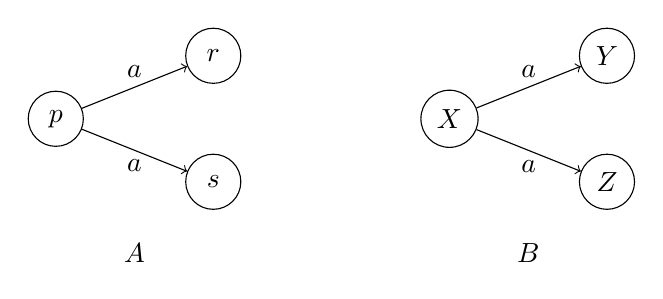
\begin{tikzpicture}[->,node distance=1.4cm]
  \tikzstyle{state}=[circle,draw,minimum size=7mm]
  \node[state] (a0) at (0,0) {$p$};
  \node[state] (a1) at (2,0.8) {$r$};
  \node[state] (a2) at (2,-0.8) {$s$};
  \node[state] (b0) at (5,0) {$X$};
  \node[state] (b1) at (7,0.8) {$Y$};
  \node[state] (b2) at (7,-0.8) {$Z$};
  \draw (a0) -- node[above] {$a$} (a1);
  \draw (a0) -- node[below] {$a$} (a2);
  \draw (b0) -- node[above] {$a$} (b1);
  \draw (b0) -- node[below] {$a$} (b2);
  \node at (1,-1.7) {$A$};
  \node at (6,-1.7) {$B$};
\end{tikzpicture}
\end{center}

\begin{block}{Subset construction during inclusion}
After reading a word $w$, we keep:
\[
  \text{one state of }A
  \qquad\text{and}\qquad
  \text{a set of possible states of }B.
\]
A counterexample to inclusion is a word that reaches acceptance in $A$ and no accepting state in $B$.
\end{block}
}
\end{frame}

\begin{frame}{Part II: finite-state bisimulation}
\Margines{
\begin{block}{Input}
A finite labelled transition system
\[
  T=(S,I,\Sigma,\to).
\]
\end{block}

\begin{block}{Output}
The bisimulation equivalence classes of states.
\end{block}

\begin{block}{Why this is useful}
The quotient transition system is smaller and satisfies the same branching-time properties invariant under bisimulation.
\end{block}
}
\end{frame}

\begin{frame}{Bisimulation as a fixed point}
\Margines{
\begin{block}{Approximants}
Let
\[
  B_0=S\times S.
\]
For $i\geq 0$, define $(s,t)\in B_{i+1}$ iff, for every $a\in\Sigma$:
\begin{itemize}
  \item if $s\xrightarrow{a}s'$, then there exists $t\xrightarrow{a}t'$ with $(s',t')\in B_i$,
  \item if $t\xrightarrow{a}t'$, then there exists $s\xrightarrow{a}s'$ with $(s',t')\in B_i$.
\end{itemize}
\end{block}

\[
  B_0\supseteq B_1\supseteq B_2\supseteq\cdots
\]

For finite systems the sequence stabilizes, and the limit is bisimilarity.
}
\end{frame}

\begin{frame}{From relations to partitions}
\Margines{
\begin{block}{Equivalence relation as a partition}
If $B$ is an equivalence relation on $S$, it partitions $S$ into equivalence classes.
\end{block}

\begin{block}{Initial partition}
For Kripke structures, start by separating states with different labels:
\[
  s\equiv_0 t
  \quad\Longleftrightarrow\quad
  L(s)=L(t).
\]
For plain LTSs without state labels, one may start with one block $S$.
\end{block}

\begin{block}{Refinement idea}
Repeatedly split blocks until all states in one block have the same one-step behaviour with respect to the current partition.
\end{block}
}
\end{frame}

\begin{frame}{Predecessor sets}
\Margines{
For a block $C\subseteq S$ and an action $a\in\Sigma$, define
\[
  \PreA_a(C)=\{s\in S : \exists t\in C\; s\xrightarrow{a}t\}.
\]

\begin{block}{Meaning}
$\PreA_a(C)$ is the set of states that can reach the block $C$ by an $a$-transition.
\end{block}

\begin{block}{When does $(a,C)$ split a block $B$?}
The block $B$ is split by $(a,C)$ if
\[
  B\cap \PreA_a(C)\neq\emptyset
  \quad\text{and}\quad
  B\setminus \PreA_a(C)\neq\emptyset.
\]
\end{block}
}
\end{frame}

\begin{frame}{Split operation}
\Margines{
\begin{block}{Definition}
Given a partition $\Part$, a block $C\in\Part$, and an action $a\in\Sigma$, replace every block $B\in\Part$ by the non-empty sets among
\[
  B_1=B\cap \PreA_a(C),
  \qquad
  B_2=B\setminus \PreA_a(C).
\]
\end{block}

\begin{block}{Intuition}
States in $B_1$ can do an $a$-move into $C$. States in $B_2$ cannot. Therefore they cannot stay bisimilar.
\end{block}
}
\end{frame}

\begin{frame}{Stable partitions}
\Margines{
\begin{block}{Stability}
A partition $\Part$ is stable if for every $a\in\Sigma$ and every block $C\in\Part$, no block $B\in\Part$ is split by $(a,C)$.
\end{block}

Equivalently, for all blocks $B,C$ and every $a\in\Sigma$, either
\[
  B\subseteq \PreA_a(C)
\]
or
\[
  B\cap \PreA_a(C)=\emptyset.
\]

\begin{block}{Theorem}
The coarsest stable refinement of the initial partition is the bisimulation quotient.
\end{block}
}
\end{frame}

\begin{frame}{Naive partition refinement algorithm}
\Margines{
\begin{enumerate}
  \item Initialize a partition $\Part$.
  \item While there exist $a\in\Sigma$ and blocks $B,C\in\Part$ such that $(a,C)$ splits $B$:
  \[
    B \quad\leadsto\quad B\cap\PreA_a(C),\quad B\setminus\PreA_a(C).
  \]
  \item Return the final partition.
\end{enumerate}

\begin{block}{Termination}
Every proper split increases the number of blocks. There are at most $|S|$ blocks.
\end{block}

\begin{block}{Correctness intuition}
At the end, states in one block can match transitions to the same blocks, and therefore the partition defines a bisimulation.
\end{block}
}
\end{frame}

\begin{frame}{Correctness: stable means bisimulation}
\Margines{
Let $\Part$ be stable. Define
\[
  s\equiv_\Part t
  \quad\Longleftrightarrow\quad
  s,t\text{ are in the same block of }\Part.
\]

\begin{block}{Claim}
$\equiv_\Part$ is a bisimulation.
\end{block}

\begin{block}{Proof idea}
Assume $s\equiv_\Part t$ and $s\xrightarrow{a}s'$. Let $C$ be the block of $s'$. Then $s\in\PreA_a(C)$. By stability, the whole block of $s$ is contained in $\PreA_a(C)$. Hence $t$ also has an $a$-successor in $C$.
\end{block}
}
\end{frame}

\begin{frame}{Correctness: why coarsest?}
\Margines{
\begin{block}{Invariant}
Every bisimulation contained in the initial partition is contained in every partition produced by the algorithm.
\end{block}

\begin{block}{Reason}
Suppose a split uses $\PreA_a(C)$. If two bisimilar states are in one block, either both can reach $C$ by an $a$-transition, or neither can. Therefore a split never separates bisimilar states.
\end{block}

\begin{block}{Conclusion}
The final stable partition is not only a bisimulation partition; it is the coarsest stable refinement, hence the bisimulation quotient.
\end{block}
}
\end{frame}

\begin{frame}{Example of one split}
\Margines{
\begin{center}
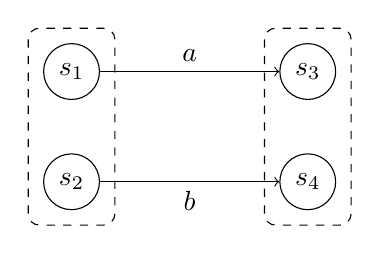
\begin{tikzpicture}[->,node distance=1.7cm]
  \tikzstyle{state}=[circle,draw,minimum size=7mm]
  \node[state] (s1) at (0,0) {$s_1$};
  \node[state] (s2) at (0,-1.4) {$s_2$};
  \node[state] (s3) at (3,0) {$s_3$};
  \node[state] (s4) at (3,-1.4) {$s_4$};
  \draw (s1) -- node[above] {$a$} (s3);
  \draw (s2) -- node[below] {$b$} (s4);
  \draw[dashed,rounded corners] (-0.55,0.55) rectangle (0.55,-1.95);
  \draw[dashed,rounded corners] (2.45,0.55) rectangle (3.55,-1.95);
\end{tikzpicture}
\end{center}

Suppose initially
\[
  \Part=\{\{s_1,s_2\},\{s_3,s_4\}\}.
\]
The block $C=\{s_3,s_4\}$ and action $a$ split $\{s_1,s_2\}$, because only $s_1$ has an $a$-transition into $C$.
\[
  \{s_1,s_2\}\quad\leadsto\quad \{s_1\},\{s_2\}.
\]
}
\end{frame}

\begin{frame}{Paige--Tarjan idea}
\Margines{
\begin{block}{Naive implementation}
The basic refinement algorithm is polynomial and sufficient for understanding the construction.
\end{block}

\begin{block}{Efficient implementation}
With suitable data structures, Paige--Tarjan partition refinement computes bisimulation in time
\[
  O(m\log n),
\]
where $n=|S|$ and $m=|\to|$.
\end{block}

\begin{block}{Main idea}
After a split, process the smaller part as a splitter. A state can belong to such a smaller splitter only $O(\log n)$ times.
\end{block}
}
\end{frame}

\begin{frame}{Part III: beyond finite-state systems}
\Margines{
\begin{block}{Finite-state case}
For finite models the situation is algorithmic:
\begin{itemize}
  \item NFA language equivalence is decidable, but PSPACE-complete;
  \item finite-state bisimulation is computable by partition refinement.
\end{itemize}
\end{block}

\begin{block}{Main message}
For even very simple infinite-state systems, the same questions usually become undecidable:
\begin{itemize}
  \item language inclusion/equivalence quickly becomes undecidable;
  \item bisimilarity also quickly becomes undecidable.
\end{itemize}
\end{block}


}
\end{frame}

\begin{frame}{One-counter nets}
\Margines{
\begin{block}{Definition}
A one-counter net is a finite-state system with one non-negative counter.
Transitions have the form
\[
  p\xrightarrow{a,d}q,
  \qquad d\in\{-1,0,1\},
\]
and transform configurations by
\[
  (p,n)\xrightarrow{a}(q,n+d)
  \quad\text{if } n+d\geq 0.
\]
\end{block}

\begin{block}{Important restriction}
There is no explicit zero test. A decrement is simply disabled at counter value $0$.
\end{block}

\begin{block}{Viewpoint}
One-counter nets are the one-dimensional case of VASS / Petri nets.
\end{block}
}
\end{frame}

\begin{frame}{Language problems for one-counter nets}
\Margines{
\begin{block}{Trace language}
The language of an OCN process is the set of words labelling paths from the initial configuration to an accepting control state.
\end{block}

\begin{block}{Undecidability border}
For nondeterministic one-counter nets, trace inclusion is undecidable. Natural language-equivalence variants for one-counter/VASS processes are also undecidable.
\end{block}

\begin{block}{Lesson}
Adding only one unbounded counter already destroys the robust decidability picture known from finite automata.
\end{block}
}
\end{frame}

\begin{frame}{A rare positive result: simulation for OCN}
\Margines{
\begin{block}{Positive result}
Simulation preorder is decidable for one-counter nets.
\end{block}

\begin{block}{Complexity landscape}
Known results place the problem at PSPACE-complete complexity.
\end{block}

\begin{block}{How to read this result}
This is an exception rather than the rule. It shows that some branching preorders can survive one unbounded counter, but it does not restore a general algorithmic theory for infinite-state equivalence checking.
\end{block}
}
\end{frame}

\begin{frame}{Petri nets and bisimulation}
\Margines{
\begin{block}{Petri net processes}
A labelled Petri net induces an infinite labelled transition system whose states are markings and whose transitions are firings.
\end{block}

\begin{block}{Jan\v{c}ar's theorem}
Bisimilarity is undecidable for labelled place/transition Petri nets.
\end{block}

\begin{block}{Interpretation}
The finite partition-refinement algorithm relies on a finite set of states. For Petri nets the reachability graph is infinite, and there is in general no computable finite quotient representing bisimilarity.
\end{block}
}
\end{frame}

\begin{frame}{Why the boundary is surprising}
\Margines{
\begin{center}
\renewcommand{\arraystretch}{1.35}
\begin{tabular}{|>{\centering\arraybackslash}m{0.31\textwidth}|>{\centering\arraybackslash}m{0.31\textwidth}|>{\centering\arraybackslash}m{0.25\textwidth}|}
\hline
model & relation/problem & status \\
\hline
finite automata & language equivalence & decidable, PSPACE-complete \\
\hline
finite LTS & bisimulation & polynomial / near-linear-log algorithms \\
\hline
one-counter nets & trace inclusion & undecidable \\
\hline
one-counter nets & simulation & decidable \\
\hline
Petri nets & bisimulation & undecidable \\
\hline
\end{tabular}
\end{center}

\begin{block}{Moral}
The practical message is negative: once we leave finite-state systems, language equivalence and bisimilarity quickly become undecidable. Decidable cases are special islands.
\end{block}
}
\end{frame}

\begin{frame}{Decidable islands}
\Margines{
\begin{center}
\renewcommand{\arraystretch}{1.35}
\begin{tabular}{|>{\raggedright\arraybackslash}m{0.42\textwidth}|>{\raggedright\arraybackslash}m{0.46\textwidth}|}
\hline
class & decidable problem \\
\hline
DPDA & language equivalence \\
\hline
pushdown processes / PDA processes & bisimulation equivalence \\
\hline
deterministic one-counter automata & language equivalence \\
\hline
one-counter nets & simulation preorder \\
\hline
deterministic Petri nets / VASS with coverability acceptance & language inclusion/equivalence in decidable fragments \\
\hline
\end{tabular}
\end{center}

\begin{block}{Important point}
Most positive results use strong structure: determinism, one-dimensionality, stack discipline, or restricted acceptance. They are important as boundary results, but usually not general-purpose verification methods.
\end{block}
}
\end{frame}

\begin{frame}{How to read decidability results}
\Margines{
\begin{block}{Three independent choices}
\begin{enumerate}
  \item The model: NFA, PDA, OCN, VASS, Petri net.
  \item The observation: language, trace inclusion, simulation, bisimulation.
  \item The acceptance semantics: final state, reachability, coverability, \Buchi.
\end{enumerate}
\end{block}

\begin{block}{Small changes can change decidability}
Examples:
\begin{itemize}
  \item deterministic vs nondeterministic automata,
  \item one counter vs two counters,
  \item reachability vs coverability acceptance,
  \item trace equivalence vs bisimulation.
\end{itemize}
\end{block}
}
\end{frame}

\begin{frame}{Take-home picture}
\Margines{
\begin{center}
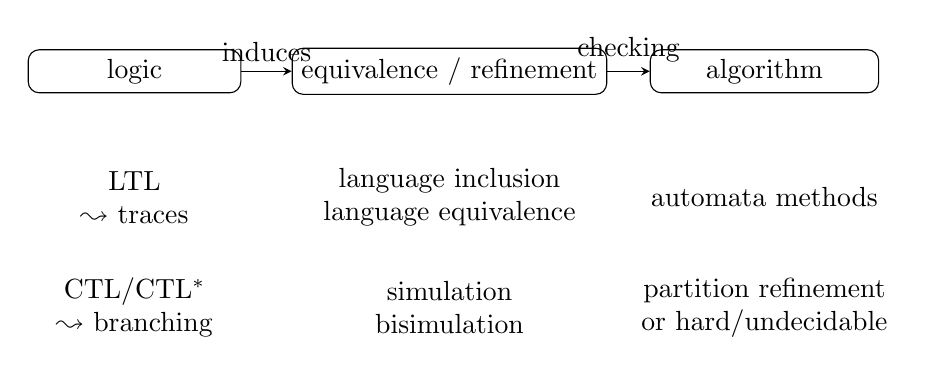
\begin{tikzpicture}[node distance=1.25cm,>=stealth]
  \node[draw,rounded corners,align=center,minimum width=2.7cm] (logic) at (0,0) {logic};
  \node[draw,rounded corners,align=center,minimum width=3.2cm] (equiv) at (4,0) {equivalence /\ refinement};
  \node[draw,rounded corners,align=center,minimum width=2.9cm] (alg) at (8,0) {algorithm};
  \draw[->] (logic) -- node[above] {induces} (equiv);
  \draw[->] (equiv) -- node[above] {checking} (alg);

  \node[align=center] at (0,-1.6) {LTL\\$\leadsto$ traces};
  \node[align=center] at (4,-1.6) {language inclusion\\language equivalence};
  \node[align=center] at (8,-1.6) {automata methods};

  \node[align=center] at (0,-3.0) {CTL/CTL$^*$\\$\leadsto$ branching};
  \node[align=center] at (4,-3.0) {simulation\\bisimulation};
  \node[align=center] at (8,-3.0) {partition refinement\\or hard/undecidable};
\end{tikzpicture}
\end{center}
}
\end{frame}

\begin{frame}{Summary}
\Margines{
\begin{itemize}
  \item Language equivalence for NFA is decidable but PSPACE-complete.
  \item Bisimulation for finite systems can be computed by partition refinement.
  \item Stability of a partition exactly captures the local matching condition of bisimulation.
  \item Infinite-state systems quickly lead to undecidability.
  \item Decidability reappears only on restricted islands; these results mostly clarify the boundary rather than give broadly practical algorithms.
\end{itemize}
}
\end{frame}

\begin{frame}{References}
\Margines{
\scriptsize
\begin{itemize}
  \item R. Paige and R. E. Tarjan. Three partition refinement algorithms. SIAM J. Comput. 16(6), 1987.
  \item P. Jan\v{c}ar. Decidability questions for bisimilarity of Petri nets and some related problems. STACS 1994 / TCS 1995.
  \item G. S\'{e}nizergues. $L(A)=L(B)$? Decidability results from complete formal systems. TCS 2001.
  \item C. Stirling. Decidability of DPDA equivalence. LFCS report, 1999.
  \item P. A. Abdulla and B. Jonsson. Simulation is decidable for one-counter nets. CONCUR 1998.
  \item P. Hofman and P. Totzke. Trace inclusion for one-counter nets revisited. TCS 2018.
  \item W. Czerwi\'{n}ski and P. Hofman. Language inclusion for boundedly-ambiguous VASS is decidable. CONCUR 2022.
\end{itemize}
}
\end{frame}

\end{document}
